% Options for packages loaded elsewhere
\PassOptionsToPackage{unicode}{hyperref}
\PassOptionsToPackage{hyphens}{url}
\PassOptionsToPackage{dvipsnames,svgnames,x11names}{xcolor}
%
\documentclass[
  11pt,
  letterpaper,
  DIV=11,
  numbers=noendperiod]{scrartcl}

\usepackage{amsmath,amssymb}
\usepackage{iftex}
\ifPDFTeX
  \usepackage[T1]{fontenc}
  \usepackage[utf8]{inputenc}
  \usepackage{textcomp} % provide euro and other symbols
\else % if luatex or xetex
  \usepackage{unicode-math}
  \defaultfontfeatures{Scale=MatchLowercase}
  \defaultfontfeatures[\rmfamily]{Ligatures=TeX,Scale=1}
\fi
\usepackage{lmodern}
\ifPDFTeX\else  
    % xetex/luatex font selection
  \setmainfont[]{Roboto}
\fi
% Use upquote if available, for straight quotes in verbatim environments
\IfFileExists{upquote.sty}{\usepackage{upquote}}{}
\IfFileExists{microtype.sty}{% use microtype if available
  \usepackage[]{microtype}
  \UseMicrotypeSet[protrusion]{basicmath} % disable protrusion for tt fonts
}{}
\makeatletter
\@ifundefined{KOMAClassName}{% if non-KOMA class
  \IfFileExists{parskip.sty}{%
    \usepackage{parskip}
  }{% else
    \setlength{\parindent}{0pt}
    \setlength{\parskip}{6pt plus 2pt minus 1pt}}
}{% if KOMA class
  \KOMAoptions{parskip=half}}
\makeatother
\usepackage{xcolor}
\usepackage[margin=1in]{geometry}
\setlength{\emergencystretch}{3em} % prevent overfull lines
\setcounter{secnumdepth}{-\maxdimen} % remove section numbering
% Make \paragraph and \subparagraph free-standing
\ifx\paragraph\undefined\else
  \let\oldparagraph\paragraph
  \renewcommand{\paragraph}[1]{\oldparagraph{#1}\mbox{}}
\fi
\ifx\subparagraph\undefined\else
  \let\oldsubparagraph\subparagraph
  \renewcommand{\subparagraph}[1]{\oldsubparagraph{#1}\mbox{}}
\fi


\providecommand{\tightlist}{%
  \setlength{\itemsep}{0pt}\setlength{\parskip}{0pt}}\usepackage{longtable,booktabs,array}
\usepackage{calc} % for calculating minipage widths
% Correct order of tables after \paragraph or \subparagraph
\usepackage{etoolbox}
\makeatletter
\patchcmd\longtable{\par}{\if@noskipsec\mbox{}\fi\par}{}{}
\makeatother
% Allow footnotes in longtable head/foot
\IfFileExists{footnotehyper.sty}{\usepackage{footnotehyper}}{\usepackage{footnote}}
\makesavenoteenv{longtable}
\usepackage{graphicx}
\makeatletter
\def\maxwidth{\ifdim\Gin@nat@width>\linewidth\linewidth\else\Gin@nat@width\fi}
\def\maxheight{\ifdim\Gin@nat@height>\textheight\textheight\else\Gin@nat@height\fi}
\makeatother
% Scale images if necessary, so that they will not overflow the page
% margins by default, and it is still possible to overwrite the defaults
% using explicit options in \includegraphics[width, height, ...]{}
\setkeys{Gin}{width=\maxwidth,height=\maxheight,keepaspectratio}
% Set default figure placement to htbp
\makeatletter
\def\fps@figure{htbp}
\makeatother
% definitions for citeproc citations
\NewDocumentCommand\citeproctext{}{}
\NewDocumentCommand\citeproc{mm}{%
  \begingroup\def\citeproctext{#2}\cite{#1}\endgroup}
\makeatletter
 % allow citations to break across lines
 \let\@cite@ofmt\@firstofone
 % avoid brackets around text for \cite:
 \def\@biblabel#1{}
 \def\@cite#1#2{{#1\if@tempswa , #2\fi}}
\makeatother
\newlength{\cslhangindent}
\setlength{\cslhangindent}{1.5em}
\newlength{\csllabelwidth}
\setlength{\csllabelwidth}{3em}
\newenvironment{CSLReferences}[2] % #1 hanging-indent, #2 entry-spacing
 {\begin{list}{}{%
  \setlength{\itemindent}{0pt}
  \setlength{\leftmargin}{0pt}
  \setlength{\parsep}{0pt}
  % turn on hanging indent if param 1 is 1
  \ifodd #1
   \setlength{\leftmargin}{\cslhangindent}
   \setlength{\itemindent}{-1\cslhangindent}
  \fi
  % set entry spacing
  \setlength{\itemsep}{#2\baselineskip}}}
 {\end{list}}
\usepackage{calc}
\newcommand{\CSLBlock}[1]{\hfill\break\parbox[t]{\linewidth}{\strut\ignorespaces#1\strut}}
\newcommand{\CSLLeftMargin}[1]{\parbox[t]{\csllabelwidth}{\strut#1\strut}}
\newcommand{\CSLRightInline}[1]{\parbox[t]{\linewidth - \csllabelwidth}{\strut#1\strut}}
\newcommand{\CSLIndent}[1]{\hspace{\cslhangindent}#1}

\KOMAoption{captions}{tableheading}
\makeatletter
\@ifpackageloaded{caption}{}{\usepackage{caption}}
\AtBeginDocument{%
\ifdefined\contentsname
  \renewcommand*\contentsname{Table of contents}
\else
  \newcommand\contentsname{Table of contents}
\fi
\ifdefined\listfigurename
  \renewcommand*\listfigurename{List of Figures}
\else
  \newcommand\listfigurename{List of Figures}
\fi
\ifdefined\listtablename
  \renewcommand*\listtablename{List of Tables}
\else
  \newcommand\listtablename{List of Tables}
\fi
\ifdefined\figurename
  \renewcommand*\figurename{Figure}
\else
  \newcommand\figurename{Figure}
\fi
\ifdefined\tablename
  \renewcommand*\tablename{Table}
\else
  \newcommand\tablename{Table}
\fi
}
\@ifpackageloaded{float}{}{\usepackage{float}}
\floatstyle{ruled}
\@ifundefined{c@chapter}{\newfloat{codelisting}{h}{lop}}{\newfloat{codelisting}{h}{lop}[chapter]}
\floatname{codelisting}{Listing}
\newcommand*\listoflistings{\listof{codelisting}{List of Listings}}
\makeatother
\makeatletter
\makeatother
\makeatletter
\@ifpackageloaded{caption}{}{\usepackage{caption}}
\@ifpackageloaded{subcaption}{}{\usepackage{subcaption}}
\makeatother
\ifLuaTeX
  \usepackage{selnolig}  % disable illegal ligatures
\fi
\usepackage{bookmark}

\IfFileExists{xurl.sty}{\usepackage{xurl}}{} % add URL line breaks if available
\urlstyle{same} % disable monospaced font for URLs
\hypersetup{
  pdftitle={An example document looking into the gender pay gap in UK companies},
  pdfauthor={Andrew Moles; Anton Boichenko},
  pdfkeywords={pandoc, r markdown, knitr},
  colorlinks=true,
  linkcolor={red},
  filecolor={Maroon},
  citecolor={Blue},
  urlcolor={blue},
  pdfcreator={LaTeX via pandoc}}

\title{An example document looking into the gender pay gap in UK
companies\thanks{Replication files are available on the
\href{https://github.com/andrewmoles2/gender_pay_gap_example}{author's
Github account}}}
\author{Andrew Moles \and Anton Boichenko}
\date{2024-07-24}

\begin{document}
\maketitle
\begin{abstract}
The gender pay gap has been an issue for generations, but how are UK
companies doing in the current climate?
\end{abstract}

\newpage

\raggedright
\newpage
\setcounter{tocdepth}{4}
\tableofcontents
\listoffigures
\listoftables

\newpage

\section{Introduction}\label{introduction}

International Women's day in 2022 was full of drama in the Twitter
world, now known as X. This was caused by the \emph{Gender Pay Gap Bot}.
Whenever a company listed on the
\href{https://gender-pay-gap.service.gov.uk/}{governments gender pay gap
service} tweets about International Women's day, the bot will
automatically respond with that company's median gender pay gap score.
It was designed to
\href{https://www.independent.co.uk/tech/people-ryanair-manchester-the-new-york-times-university-b2296194.html}{pressure
on companies to be accountable} for gender equality.

\begin{figure}[H]

{\centering 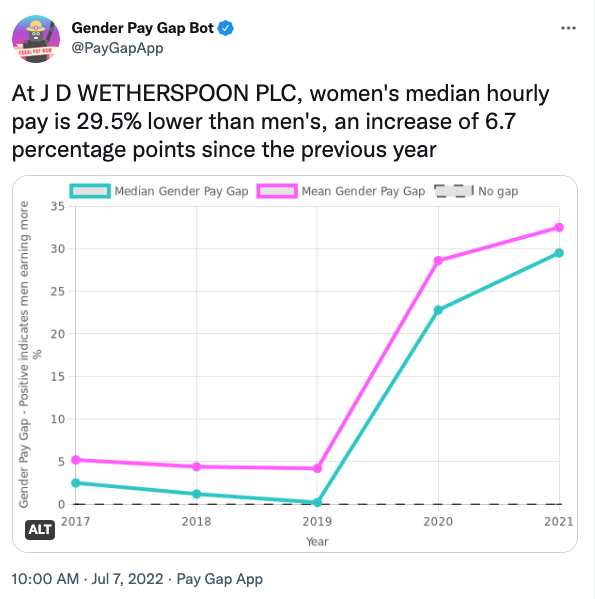
\includegraphics[width=0.7\textwidth,height=\textheight]{pay_gap_bot.png}

}

\caption{The gender pay gap bot in action}

\end{figure}%

The bot caused a lot of companies to remove their tweets and even post
some amendments. The point of the project was to call out companies that
talked a good talk but had very poor gender pay equality.

This report wanted to look more into the governments gender pay gap
service data to see if we could see any extra insights or interesting
patterns.

\newpage

\section{Methods}\label{methods}

The data used for this report is from the UK
\href{https://gender-pay-gap.service.gov.uk/}{governments gender pay gap
service}. This data has been helpfully hosted and joined together by
\href{https://github.com/rfordatascience/tidytuesday/tree/master/data/2022/2022-06-28}{the
TidyTuesday project}.

There are several variables of interest which we can use in an analysis
of this data: DiffMeanHourlyPercent, DiffMedianHourlyPercent, PostCode,
SicCodes, and EmployerSize.

DiffMeanHourlyPercent and DiffMedianHourlyPercent are the mean or median
\% difference between male and female hourly pay (negative = women's
mean/median hourly pay is higher). PostCode is each companies postal
code. SicCodes are used to describe the employer's purpose and sectors
of work at the time of reporting, e.g.~the company is in the finance
sector. EmployerSize indicates the number of employers which is grouped
into bands such as \emph{250 to 499} or \emph{5000 to 19,999}.

The formula used to calculate the DiffMeanHourlyPercent and
DiffMedianHourlyPercent columns is as follows:

\[ {{value_{original} - value_{new}} \over {value_{original}}} \times 100 \]

If females are paid better, the data will show a minus value for that
column. This is because the original value in the formula is male as
shown below:
\[ {{male\_wage - female\_wage \over male\_wage}} \times 100 \]

In the analysis of the data several R packages were used which are: the
tidyverse (Wickham et al. 2019), tidytext (Silge and Robinson 2016),
ggtext (Wilke 2020), patchwork (Pedersen 2020), geogrid (Bailey 2018),
rmapshaper (Teucher and Russell 2022), and sf (Pebesma 2018).

\newpage

\section{Results}\label{results}

We can first look at the sector averages, here we are looking at the top
10 sectors that have, on average, the largest percent gap in men's wages
compared to women's wages. To get the sectors, Tokenisation\footnote{Tokenisation
  is a way of separating text into smaller units called \emph{tokens},
  which can be either words, characters or sub words.} of Standard
industrial classification of economic activities (SIC) codes was used in
an attempted to simplify the results.

\begin{longtable}[]{@{}lc@{}}
\caption{Table to show the sectors with, on average, the largest percent
gap in men's wages compared to women's wages.}\tabularnewline
\toprule\noalign{}
\textbf{sector} & \textbf{percent increase in mens wages compared to
womens} \\
\midrule\noalign{}
\endfirsthead
\toprule\noalign{}
\textbf{sector} & \textbf{percent increase in mens wages compared to
womens} \\
\midrule\noalign{}
\endhead
\bottomrule\noalign{}
\endlastfoot
primary & 0.2835 \\
secondary & 0.2494 \\
education & 0.2383 \\
financial & 0.2112 \\
construction & 0.1978 \\
technology & 0.1932 \\
information & 0.1892 \\
head & 0.164 \\
offices & 0.164 \\
technical & 0.1615 \\
\end{longtable}

Ideas for this analysis were taken from from this blog post by
\href{https://juliasilge.com/blog/pay-gap-uk/}{Julia Silge}.

A more elaborate analysis we can do is to look at the gender pay gap by
company size and by postcode area. Figure \ref{fig:makefigure} gives us
an overall general picture of this difference by area. The clearest
outcome here is that most of the grids for all employee sizes are green
or black, the black hexagons indicating missing data for the postcode
area. There are seemingly some areas where this isn't so much the case,
which seem to be around Lancashire and Northumberland.

The code for Figure \ref{fig:makefigure} came from
\href{https://github.com/gkaramanis/tidytuesday/tree/master/2022/2022-week_26}{Georgios
Karamandis} as a Tidy Tuesday contribution.

\begin{figure}[H]

{\centering 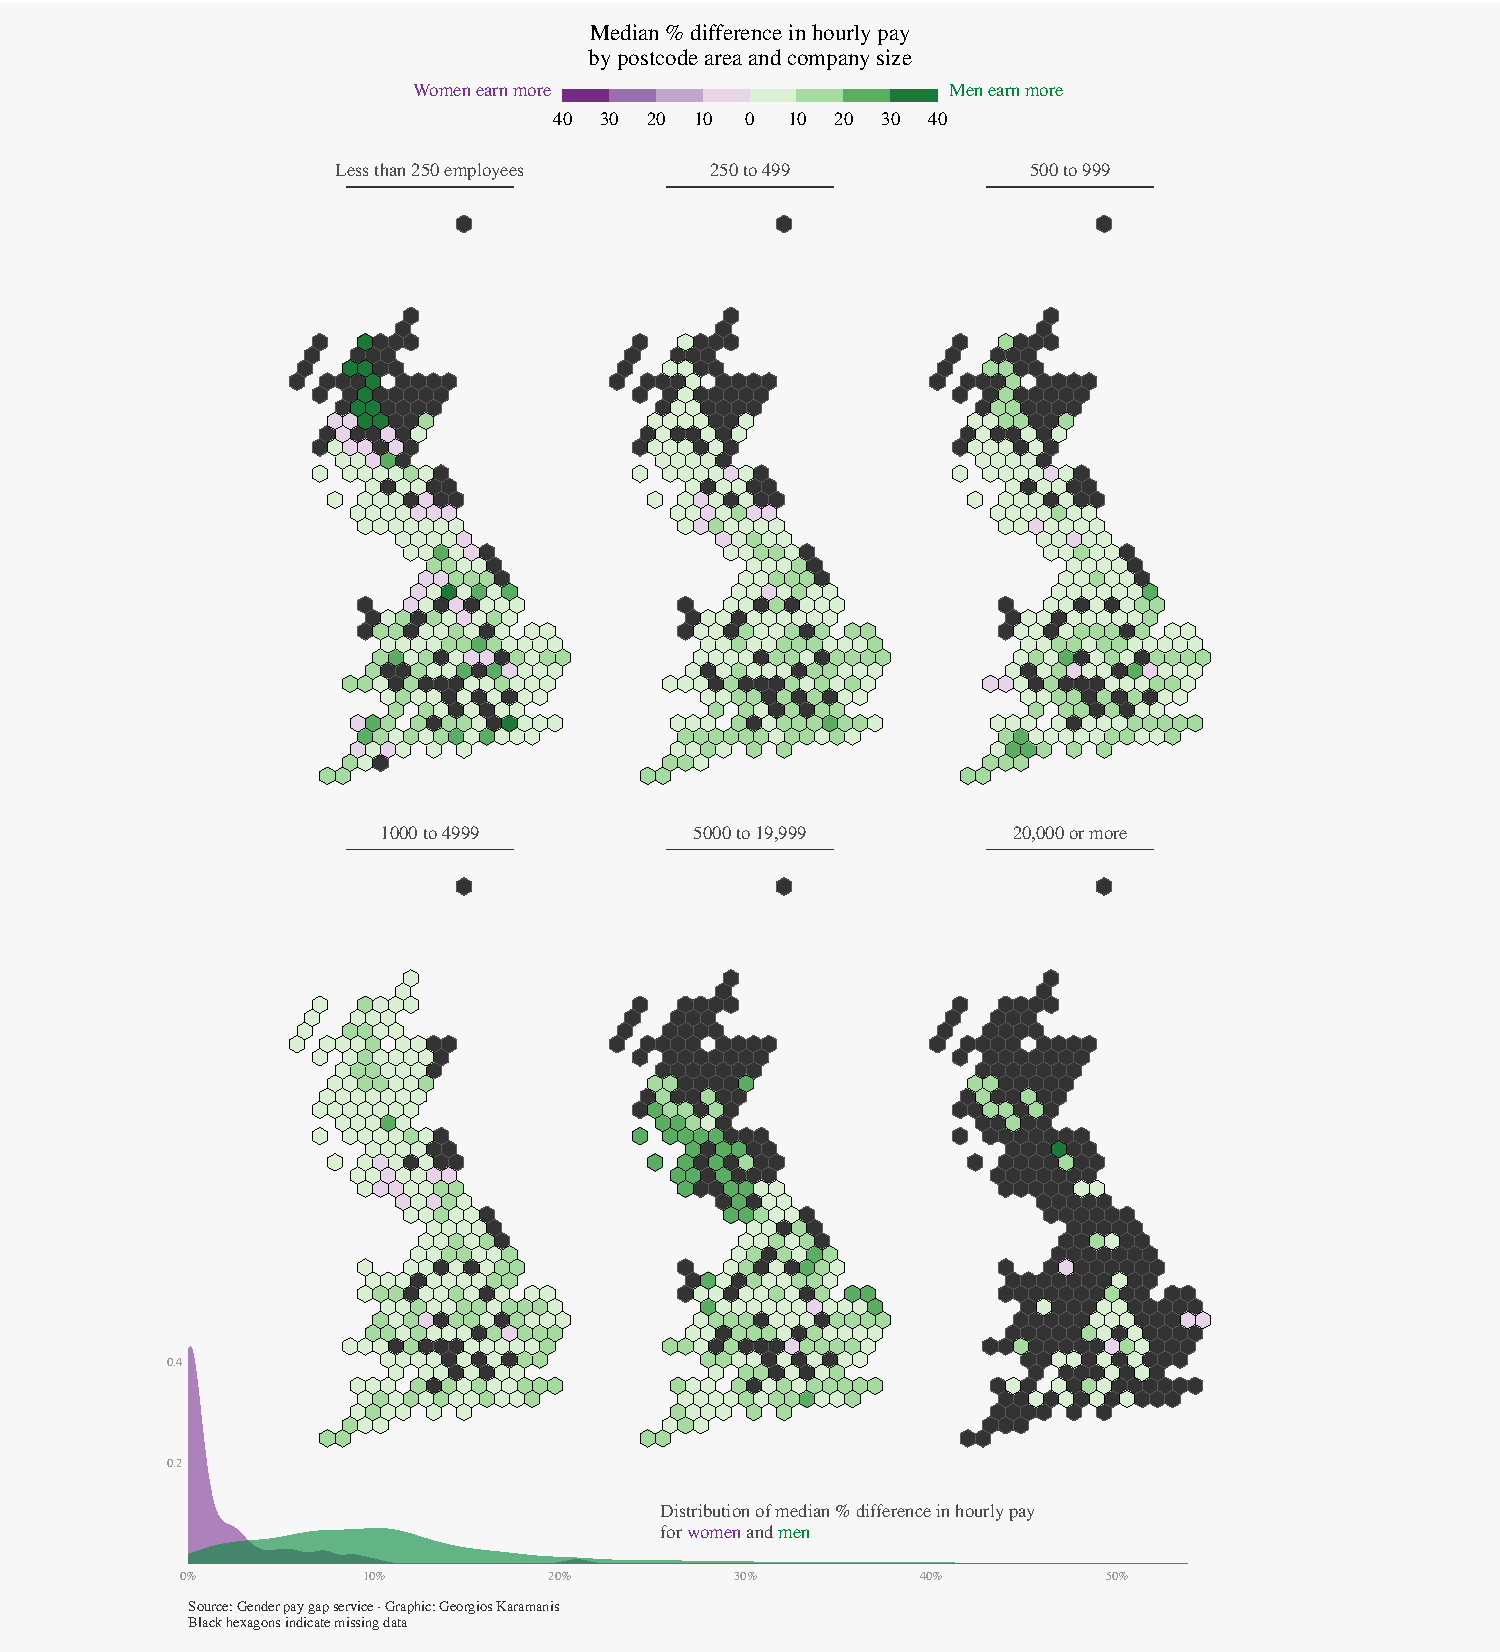
\includegraphics[width=0.8\textwidth,height=\textheight]{gender_pay_gap_files/figure-pdf/geomaps-1.pdf}

}

\caption{\label{fig:makefigure} Median percentage difference in hourly
pay by postcode area and company size}

\end{figure}%

\newpage

\section{Discussion}\label{discussion}

Theresa May, in her first statement as Prime Minister highlighted that:

\begin{quote}
``If you're a woman, you will earn less than a man.''
\end{quote}

Our results show that on average, this is still the case but there are a
lot of caveats.

Pay between genders is complicated as it does vary over a lifetime. It
can differ depending on whether you are looking at full-time or
part-time working (or both), what age you are, what ethnicity you are
and your seniority within an occupation. For example there may be a
wider (or narrower) GPG in those earning a higher salary as an actor
than in those earning a lower salary.

It's also important to consider the ratio of men to women in each
occupation and whether any difference is due to one gender being
disadvantaged in this field or whether they are just naturally more or
less inclined go into that type of work\footnote{This text was taken
  from
  \href{https://www.ons.gov.uk/employmentandlabourmarket/peopleinwork/earningsandworkinghours/articles/testyourknowledgeonthegenderpaygap/2016-12-09}{ONS
  gender pay gap web pages}}.

The reasons for the gender pay gap are complex and overlapping:

\begin{itemize}
\item
  girls do well at school but often choose occupations or sectors that
  offer narrower scope for financial reward - many of the highest paying
  sectors are disproportionately made up of male employees.
\item
  a proportion of the gap may be due to the negative effect on wages of
  having worked part-time or having taken time out of the labour market
  to look after family.
\item
  women may not progress in work at the same rate as men due to cultural
  attitudes, lack of flexible working and stereotyping.
\item
  some older women may need to learn new skills to take advantage of
  employment opportunities in growing sectors; others may have increased
  caring responsibilities for partners, grandchildren or ageing parents.
\end{itemize}

\newpage

\phantomsection\label{refs}
\begin{CSLReferences}{1}{0}
\bibitem[\citeproctext]{ref-geogrid}
Bailey, Joseph. 2018. \emph{Geogrid: Turn Geospatial Polygons into
Regular or Hexagonal Grids}.
\url{https://CRAN.R-project.org/package=geogrid}.

\bibitem[\citeproctext]{ref-sf}
Pebesma, Edzer. 2018. {``{Simple Features for R: Standardized Support
for Spatial Vector Data}.''} \emph{{The R Journal}} 10 (1): 439--46.
\url{https://doi.org/10.32614/RJ-2018-009}.

\bibitem[\citeproctext]{ref-patchwork}
Pedersen, Thomas Lin. 2020. \emph{Patchwork: The Composer of Plots}.
\url{https://CRAN.R-project.org/package=patchwork}.

\bibitem[\citeproctext]{ref-tidytext}
Silge, Julia, and David Robinson. 2016. {``Tidytext: Text Mining and
Analysis Using Tidy Data Principles in r.''} \emph{JOSS} 1 (3).
\url{https://doi.org/10.21105/joss.00037}.

\bibitem[\citeproctext]{ref-rmapshaper}
Teucher, Andy, and Kenton Russell. 2022. \emph{Rmapshaper: Client for
'Mapshaper' for 'Geospatial' Operations}.
\url{https://CRAN.R-project.org/package=rmapshaper}.

\bibitem[\citeproctext]{ref-tidyverse}
Wickham, Hadley, Mara Averick, Jennifer Bryan, Winston Chang, Lucy
D'Agostino McGowan, Romain François, Garrett Grolemund, et al. 2019.
{``Welcome to the {tidyverse}.''} \emph{Journal of Open Source Software}
4 (43): 1686. \url{https://doi.org/10.21105/joss.01686}.

\bibitem[\citeproctext]{ref-ggtext}
Wilke, Claus O. 2020. \emph{Ggtext: Improved Text Rendering Support for
'Ggplot2'}. \url{https://CRAN.R-project.org/package=ggtext}.

\end{CSLReferences}



\end{document}
